\tikzset{
label/.style={
  rectangle,
  draw=none,
  text centered,
  inner sep=0em,
},
}

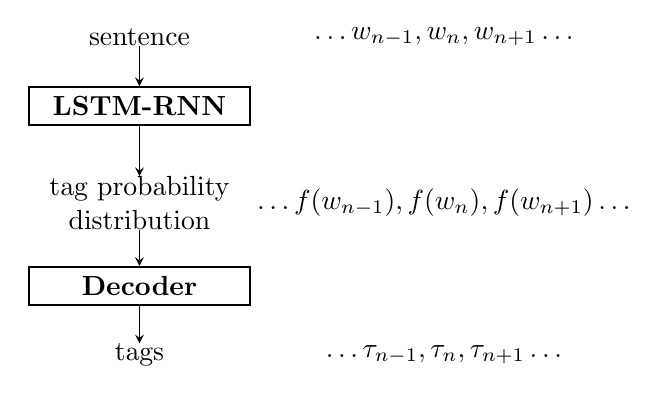
\begin{tikzpicture}[x=1em, y=1em, >=stealth]
%block1
%outer block
\node[label](input) at (0,0) {sentence};
\node[label](inputsample) at (11,0) {$\dots w_{n-1}, w_{n}, w_{n+1} \dots$};
\node[rectangle,draw, minimum width=8em, thick](BLSTM) at (0,-2.5){\textbf{LSTM-RNN}};
\node[label, text width=8em](ioutput) at (0,-6) {tag probability distribution};
\node[label](ioutputsample) at (11,-6) {$\dots f(w_{n-1}), f(w_{n}), f(w_{n+1}) \dots$};
\node[rectangle,draw, minimum width=8em, thick](Decoder) at (0,-9){\textbf{Decoder}};
\node[label, text width=8em](output) at (0,-11.5) {tags};
\node[label](inputsample) at (11,-11.5) {$\dots \tau_{n-1}, \tau_{n}, \tau_{n+1} \dots$};

\draw[->](input) -- (BLSTM);
\draw[->](BLSTM) -- (ioutput);
\draw[->](ioutput) -- (Decoder);
\draw[->](Decoder) -- (output);

\end{tikzpicture} 
